% Template created by Karol Kozioł (www.karol-koziol.net) for ShareLaTeX

\documentclass[a4paper,9pt]{extarticle}
\usepackage[utf8]{inputenc}
\usepackage[T1]{fontenc}
\usepackage{graphicx}
\usepackage{xcolor}
\usepackage{tikz}

\usepackage{listings}
\lstset{basicstyle=\ttfamily,
  showstringspaces=false,
  commentstyle=\color{red},
  keywordstyle=\color{blue}
}



\usepackage{amsmath,amssymb,textcomp}
\everymath{\displaystyle}

\usepackage{times}
\renewcommand\familydefault{\sfdefault}
\usepackage{tgheros}
\usepackage[defaultmono,scale=0.85]{droidmono}

\usepackage{multicol}
\setlength{\columnseprule}{0pt}
\setlength{\columnsep}{20.0pt}


\usepackage{geometry}
\geometry{
a4paper,
total={210mm,297mm},
left=10mm,right=10mm,top=10mm,bottom=15mm}

\linespread{1.3}


% custom title
\makeatletter
\renewcommand*{\maketitle}{%
\noindent
\begin{minipage}{0.4\textwidth}

\begin{tikzpicture}
\node[rectangle,rounded corners=6pt,inner sep=10pt,fill=blue!60!green,text width= 0.95\textwidth] {\color{white}\Huge \bf \@title};
\end{tikzpicture}
\end{minipage}
\hfill
\begin{minipage}{0.55\textwidth}
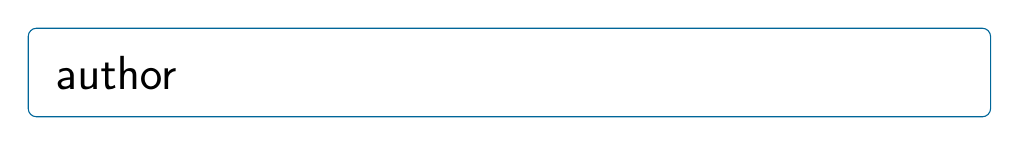
\begin{tikzpicture}
\node[rectangle,rounded corners=3pt,inner sep=10pt,draw=blue!60!green,text width= 0.95\textwidth] {\LARGE \@author};
\end{tikzpicture}
\end{minipage}
\bigskip\bigskip
}%
\makeatother

% custom section
\usepackage[explicit]{titlesec}
\newcommand*\sectionlabel{}
\titleformat{\section}
  {\gdef\sectionlabel{}
   \normalfont\sffamily\Large\bfseries\scshape}
  {\gdef\sectionlabel{\thesection\ }}{0pt}
  {
\noindent
\begin{tikzpicture}
\node[rectangle,rounded corners=3pt,inner sep=4pt,fill=blue!60!green,text width= 0.95\columnwidth] {\color{white}\sectionlabel#1};
\end{tikzpicture}
  }
\titlespacing*{\section}{0pt}{15pt}{10pt}


% custom footer
\usepackage{fancyhdr}
\makeatletter
\pagestyle{fancy}
\fancyhead{}
\fancyfoot[C]{\footnotesize \textcopyright\ \@author. \ \@date}
\renewcommand{\headrulewidth}{0pt}
\renewcommand{\footrulewidth}{0pt}
\makeatother


\title{Command Line (Linux) CheatSheet \normalsize \textit{for my simple need}}
\author{Fawaz Alazemi}
\date{Last update:\today}



\begin{document}

\maketitle
\begin{multicols*}{2}
\section{Misc}
\textbf{\large Delete files matching x in current and subdirectories  }
\begin{lstlisting}[language=bash]
$ find . -type f -name 'x' -delete
\end{lstlisting}
\textbf{\large Download a file from internet}
\begin{lstlisting}[language=bash]
$ wget URL
\end{lstlisting}
\textbf{\large Remove all temp files after make}
\begin{lstlisting}[language=bash]
$ make clean
\end{lstlisting}





\section{Grep}
\textbf{\large Search for a specific string in a list of files}
\begin{lstlisting}[language=bash]
$ grep "TEXT" *.cpp
\end{lstlisting}
\textbf{\large To recursively search for a pattern in a path directory and subdirectory}
\begin{lstlisting}[language=bash]
grep -r 'path' -e "pattern"
\end{lstlisting}
\textbf{\large To show line number }
\begin{lstlisting}[language=bash]
grep -n "pattern" file
\end{lstlisting}
\textbf{\large Ignore case}
\begin{lstlisting}[language=bash]
grep -i "pattern" file
\end{lstlisting}
\textbf{\large Whole word}
\begin{lstlisting}[language=bash]
grep -w "pattern" file
\end{lstlisting}
\textbf{\large To list only file names that include the pattern}
\begin{lstlisting}[language=bash]
grep -l "pattern" file
\end{lstlisting}
\textbf{\large Example, search for x in current and sub directories}
\begin{lstlisting}[language=bash]
grep -rnw '.' -e "x"
\end{lstlisting}


\end{multicols*}

\end{document}
